\section*{Falta de água no IME}
\autoria{anônimo}
\avisoTextoForms

Desde o ano de ingresso, sempre estudei de manhã como estudante do diurno. Neste último semestre, por conta de forças maiores e circunstâncias de vida, acabei tendo que pegar matérias de noite. Além do horário de aulas e horas de sono, muitas outras coisas que nunca imaginei ser o caso mudaram também. O transporte público na ida deixou de ser a superlotação das 6 da manhã. Em compensação, no entanto, o transporte de volta virou uma corrida contra o tempo, uma vez que o metrô fecha meia-noite - e a escassez de Circulares durante o período noturno não ajuda -. A disposição para fazer qualquer atividade durante a semana mudou, já que agora parece que meus dias não rendem tanto pela perda do período de tarde livre. Estar em uma sala de aula com pessoas novas e que nunca vi na vida também foi algo que, mesmo tendo a ciência de que aconteceria, foi um pequeno choque de qualquer forma.

Houveram muitos dias em que fui olhar o cardápio dos bandejões de almoço ao invés do jantar. Mas mesmo quando lendo o cardápio certo, às vezes simplesmente não conseguia chegar a tempo de comer e assistir às aulas, e o fechamento da lanchonete às 21h faz com que não seja possível comer algo durante a troca de aulas no mesmo horário. Sobre isso, algo que tem ajudado muito, nesse sentido, foi o CAMat ter ampliado sua gama de alimentos para venda.

A inspiração para a escrita desse texto, no entanto, veio após ter saído da aula numa sexta-feira, ido ao banheiro, e perceber que não tinha água na torneira para lavar as mãos. Passei em todos os banheiros, e o mesmo se repetiu em todas as pias de todos os banheiros do Bloco B. No fim, consegui lavar as mãos somente no banheiro do Bloco A. Como nunca tinha acontecido isso comigo, fui conversar com meus veteranos sobre, mas ninguém pareceu surpreso com o fato, e pareceu ser algo que simplesmente acontece.

Por curiosidade, fui atrás para tentar entender melhor a situação, e descobri que, não só como é um problema que existe desde muito antes do meu ingresso, como também é um problema conhecido, como mostra o repasse abaixo datada de 2020, encontrado no Telegram do CAMat:

“A falta de água, no período noturno, nos bebedouros do bloco B é um problema que se fez recorrente nos últimos semestres e o qual não obtínhamos quaisquer explicação por parte da diretoria do IME. Contudo, no último Conselho Técnico Administrativo (05/03), foi informado que a origem da falta de água é a SABESP, que diminui a pressão à noite, e que a equipe de manutenção do IME já está buscando resolver o problema - seja diretamente com a SABESP ou internamente. Além disso, foi pontuado que ainda nesse ano (2020) será instalada uma caixa d’água no bloco B - requerimento do corpo de bombeiros -, o que ajudará a solucionar o problema.”

\begin{figure}[H]
    \centering
    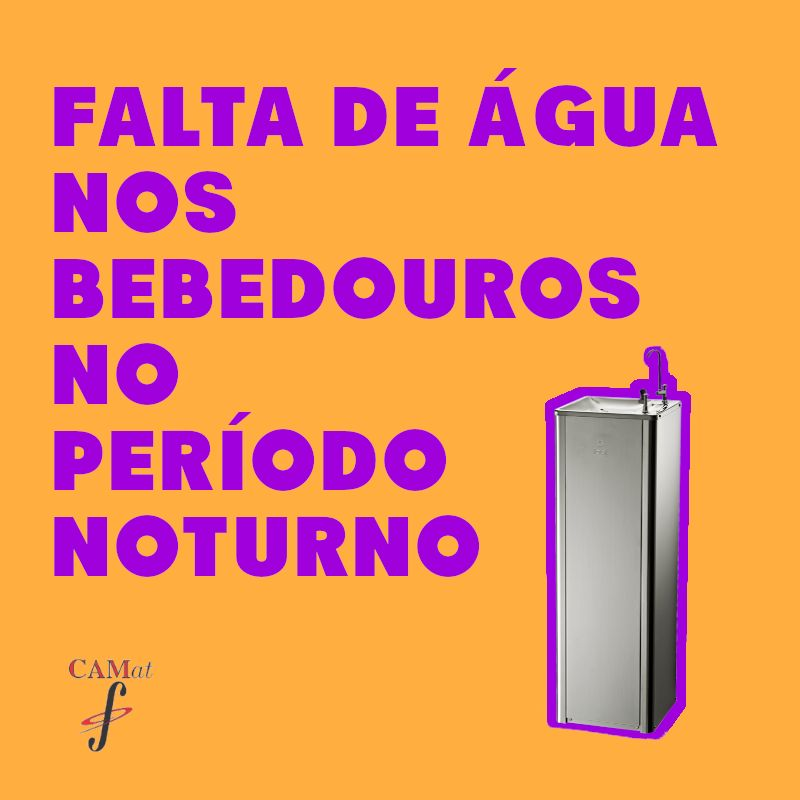
\includegraphics[width=0.65\linewidth]{textos/img/post_telegram_camat.jpg}
    \\
    \legendaFigura{1}{\textit{post do telegram} \legendaFiguraQuebraLinha Acervo CAMat}
    \vspace{-0.5cm}
\end{figure}

Quando converso esporadicamente com meus amigos do diurno - e que continuaram no diurno -, nenhuma dessas questões parecem ser evidentes para eles, do mesmo jeito que não foi evidente para mim antes de eu ter tido a necessidade de vir para noturno. Grande parte dessa separação, ao meu ver, se dá pela distância que existe entre as turmas do diurno e noturno. Não existe um diálogo muito forte entre as duas. São pessoas que vivem em realidades diferentes com necessidades diferentes. Como exemplo disso, lembro que na minha sala do diurno, poucos trabalhavam, ao ponto que na minha sala do noturno, trabalhar e depois vir para aula parece ser a regra. Isso, claro, não é uma crítica ao diurno, tampouco estou colocando juízo de valores. Apenas exponho que, na minha percepção, existem essas realidades diferentes, e que acredito ser importante para que, enquanto imeanos, entendermos a existência das outras realidades dos ambientes que frequentamos.